\documentclass[12pt]{article}

\usepackage[utf8]{inputenc}
\usepackage[T1]{fontenc}
\usepackage{amsmath,amssymb}
\usepackage{graphicx}
\usepackage[margin=2.5cm]{geometry}
\usepackage{booktabs}
\usepackage{setspace}
\usepackage{float}
\usepackage{xcolor}
\usepackage[colorlinks=true,linkcolor=blue,citecolor=blue,urlcolor=blue]{hyperref}

\newcommand{\add}[1]{\textcolor{red}{#1}}

\setlength{\parindent}{0pt}
\setlength{\parskip}{6pt}
\setstretch{1.5}
\renewcommand{\thetable}{\Roman{table}}
\makeatletter
\renewcommand{\@biblabel}[1]{}
\makeatother

\title{\bfseries Conditional Ablation of Surrogate Error in Bayesian Inversion}
\author{Rongwang Yin$^{1}$, Shaowei Zhang$^{2,*}$\\[4pt]
\small $^1$Basic Experiment and Training Center, Hefei University, Hefei 230601, P.R. China\\
\small $^2$School of Computer Engineering, AnHui WenDa University of Information Engineering, HeFei 231201, P.R. China\\
\small $^*$Corresponding author. E-mail: swzhang189@163.com}
\date{}

\begin{document}
\maketitle

\begin{abstract}
\noindent\textbf{Purpose}\\
Bayesian inversion of PDE-constrained problems increasingly relies on learned surrogates, yet surrogate-induced error is almost always assessed as a single lump sum. This paper develops a conditional ablation framework that \add{isolates how a \emph{single} surrogate property, the spectral attenuation of the forward operator, drives posterior degradation}.

\noindent\textbf{Design/methodology/approach}\\
Sensitivity is measured through three complementary diagnostics: energy distance between posterior ensembles, cosine similarity of the log-likelihood gradient, and cross-spectral Wiener analysis. A controlled frequency-attenuated surrogate with an exactly known roll-off is applied to steady-state pressure inversion on the SPE10 permeability benchmark, with multiple independent chains per configuration.

\noindent\textbf{Findings}\\
Stronger frequency attenuation consistently enlarges the energy distance to the reference posterior, and the gradient cosine similarity between surrogate-driven and reference gradients falls monotonically with attenuation. \add{A cross-spectral Wiener calibration raises the gradient cosine from $0.83$ to $0.88$ on held-out data, confirming that compensation succeeds in the high-coherence frequency bands that carry the most reference energy.}

\noindent\textbf{Originality/value}\\
Conditional ablation turns surrogate error from a single number into a structured diagnostic that directs engineering effort toward the most impactful surrogate property. The framework is demonstrated on a CPU prototype and is architected for extension to GPU-trained neural surrogates and full-physics reservoir simulators. All code and protocols are released as open source.

\medskip
\noindent\textbf{Keywords:} Bayesian inversion; surrogate modeling; ablation analysis; uncertainty quantification

\medskip
\noindent\textbf{Paper type:} Research paper
\end{abstract}

\section{Introduction}

Bayesian inversion of PDE-constrained problems requires characterizing the posterior distribution $p(x|y)\propto p(y|x)\,p(x)$ over high-dimensional parameter fields given indirect, noisy observations. In subsurface flow modeling, the canonical example is reservoir history matching: inferring permeability and porosity fields from production data. The forward model $\mathcal{F}:x\mapsto y$ solves coupled nonlinear PDEs, requiring minutes to hours per evaluation, making exhaustive posterior exploration via Markov chain Monte Carlo (MCMC) computationally prohibitive.

Learned surrogates bring practical gradient-based Bayesian inversion closer to routine use, but evaluating such pipelines end-to-end entangles several distinct error sources: surrogate approximation error, prior model mismatch, sampling bias, and finite-sample noise are all lumped into a single quality metric. When the final posterior looks wrong, the practitioner cannot trace the problem to its root cause.

We address this diagnostic gap with a conditional ablation framework. The idea is to vary one surrogate property at a time while holding the others fixed, and to measure how the posterior responds. The resulting sensitivity profile identifies which surrogate properties matter most and where engineering effort should be concentrated.

\textbf{Contributions.} (1) A formal conditional-ablation protocol for surrogate-guided Bayesian inversion, spanning distribution-level, gradient-level, and spectral diagnostics. (2) A controlled experimental design (a frequency-attenuated surrogate with an exactly known roll-off) that eliminates the confounds inherent in comparing different trained neural surrogates. (3) A cross-spectral Wiener calibration, \add{proposed with a held-out gradient-alignment validation}. (4) An open-source reference implementation tested on the SPE10 permeability benchmark.

\textbf{Scope and limitations.} This is a methodological framework paper, not an applied reservoir-characterization study. The surrogate is a deliberately simplified frequency-attenuated operator, so the attenuation level is a controlled experimental variable rather than a learned property. \add{The study is a one-dimensional spectral-attenuation sensitivity analysis: it sweeps a single, exactly known roll-off parameter and characterizes its effect on the posterior.} All computation runs on CPU with publicly available data; extending the framework to GPU-trained neural surrogates and full-physics simulators is a natural next step.

\section{Related Work}

\subsection{Learned surrogates for Bayesian inversion}

Fourier neural operators (Li et al., 2021) and their enhanced variants (Wen et al., 2022) learn mappings between function spaces. Generative priors built on variational autoencoders (Kingma and Welling, 2014), generative adversarial networks (Laloy et al., 2018), and diffusion models (Ho et al., 2020; Chung et al., 2023; Song et al., 2021) supply rich geological constraints, and simulation-based inference (Cranmer et al., 2020) amortizes posterior estimation across observations. Surrogate-assisted history matching with such operators has been demonstrated on benchmark reservoirs (Etienam et al., 2024).

\subsection{Surrogate error and the posterior}

When a surrogate stands in for the forward model, its error propagates into the posterior. Bayesian model discrepancy quantifies the simulator-to-reality gap (Kennedy and O'Hagan, 2001); adaptive surrogate construction targets accuracy where the posterior needs it (Li and Marzouk, 2014); and posterior approximation-error analysis characterizes the effect of discretization and model reduction (Cotter et al., 2009; Kaipio and Somersalo, 2007). These works reduce surrogate error or quantify a posterior for a specific surrogate.

\subsection{Ablation and spectral analysis}

The present work also builds on two diagnostics literatures. Component ablation is a standard machine-learning tool for identifying what drives model performance, and the spectral bias of neural networks shows that trained surrogates preferentially learn low-frequency components (Rahaman et al., 2019). The key difference here is control: the attenuation is set by a parameter rather than learned, so the effect of spectral truncation on the posterior can be isolated and measured directly.

\section{Method}

\subsection{Pipeline and Surrogate Model}

We consider the Metropolis-adjusted Langevin algorithm (MALA) targeting $p(x|y)\propto p(y|x)\,p(x)$. The proposal is
\begin{equation}
x^{*}=x_{t}+\frac{\epsilon^{2}}{2}\nabla_{x}\log p(x_{t}|y;G)+\epsilon\,\eta_{t},\qquad \eta_{t}\sim\mathcal{N}(0,I),
\end{equation}
where $\nabla_{x}\log p(x_{t}|y;G)=\nabla_{x}\log p(y|x_{t};G)+\nabla_{x}\log p(x_{t})$. The proposal density is $q(x^{*}|x_{t})=\mathcal{N}\big(x^{*}\,\big|\;x_{t}+\tfrac{\epsilon^{2}}{2}\nabla\log p(x_{t}|y;G),\;\epsilon^{2}I\big)$, and the Metropolis--Hastings acceptance probability is
\begin{equation}
\alpha(x_{t},x^{*})=\min\left(1,\ \frac{p(x^{*}|y;G)\,q(x_{t}|x^{*})}{p(x_{t}|y;G)\,q(x^{*}|x_{t})}\right).
\end{equation}
The step size $\epsilon$ is tuned adaptively during burn-in to achieve $50$--$80\%$ acceptance. The reference sampler uses the full forward model $\mathcal{F}$ in place of $G$.

\add{The parameter field is sampled in \emph{whitened} coordinates. Writing the Gaussian prior as $p(x)=\mathcal{N}(\mu,C)$, we set $w=C^{-1/2}(x-\mu)$, so that $w\sim\mathcal{N}(0,I)$ and MALA proposals are generated in $w$-space. The whitening operator $C^{-1/2}$ and its inverse are applied by Fourier multiplication on the regular grid, which keeps the preconditioned sampling exact and $O(n\log n)$ even for large fields.}

Our controlled surrogate \add{attenuates the \emph{parameter} field (log-permeability) before the forward solve}:
\begin{equation}
{\color{red} G_{\alpha}(x)=\mathcal{F}\big(L_{\alpha}(x)\big),\qquad L_{\alpha}(x)=\mathcal{F}^{-1}\!\big(H_{\alpha}(|\xi|)\cdot\hat{x}(\xi)\big),\qquad H_{\alpha}(|\xi|)=\exp\!\left(-\frac{|\xi|}{\alpha\,\xi_{0}}\right),}
\end{equation}
where $\mathcal{F}$ denotes the forward model, $\hat{x}=\mathcal{F}_{\mathrm{FT}}(x)$ is the Fourier transform of the parameter field, and $\xi_{0}$ is a roll-off wavenumber set to approximately one-fifth of the Nyquist frequency (grid-relative). The attenuation is exponential in wavenumber: smaller $\alpha$ gives stronger high-frequency roll-off. The limit $\alpha\to\infty$ recovers $H_{\alpha}\to1$ (no attenuation). We test $\alpha\in\{2,4,8\}$; $\alpha=2$ is the most heavily attenuated (worst surrogate) and $\alpha=8$ the least. This models a surrogate that can only represent low-frequency permeability structure (spectral truncation). \add{Because the low-pass filter $L_{\alpha}$ is linear and self-adjoint, the surrogate likelihood gradient is obtained by attenuating the reference gradient evaluated at the attenuated parameter,}
\begin{equation}
{\color{red} \nabla_{x}\log p(y|x;G_{\alpha})=L_{\alpha}\!\big(\nabla_{\tilde x}\log p(y|\tilde x)\big),\qquad \tilde x=L_{\alpha}(x).}
\end{equation}

\textbf{Important:} this controlled surrogate does \emph{not} reduce computational cost; it requires the full forward solve plus an FFT pair. Its purpose is to isolate the spectral attenuation mechanism for diagnostic analysis, not to provide speedup. Production surrogates (trained neural operators) provide the speedup, which is separate from the spectral-fidelity question studied here.

\subsection{Ablation Protocol}

For a surrogate property $\phi$, the conditional ablation effect is
\begin{equation}
\Delta(\phi_{1},\phi_{2})=D\big(p_{\phi_{1}},\,p_{\phi_{2}}\big),
\end{equation}
where $D$ is the energy distance between posterior ensembles (Sz\'ekely and Rizzo, 2013, 2017). For gradient-level comparison we decompose similarity by radial frequency band. Let $\Pi_{b}$ denote the projection onto the annulus $b\le|k|<b+1$. The bandwise cosine similarity is
\begin{equation}
\cos_{b}(\hat g,g^{*})=\frac{\operatorname{Re}\langle\Pi_{b}\hat g,\ \Pi_{b}g^{*}\rangle}{\|\Pi_{b}\hat g\|_{2}\cdot\|\Pi_{b}g^{*}\|_{2}+\epsilon_{c}},\qquad \epsilon_{c}=10^{-8},
\end{equation}
where $\langle u,v\rangle=\sum_{k}\mathcal{F}(u)(k)\cdot[\mathcal{F}(v)(k)]^{*}$ is the $\ell_{2}$ inner product with complex conjugation in the second argument. The scalar cosine $\overline{\cos}$ reported below is the gradient-energy-weighted average across bands,
\begin{equation}
\overline{\cos}=\frac{\sum_{b}\|\Pi_{b}g^{*}\|_{2}^{2}\cdot\cos_{b}}{\sum_{b}\|\Pi_{b}g^{*}\|_{2}^{2}}.
\end{equation}

\subsection{Convergence Diagnostics}

All experiments use multiple independent MALA chains per configuration. We report the maximum Gelman--Rubin $\hat R$ across the posterior field components and the minimum effective sample size (ESS). Energy-distance bootstrap confidence intervals use $1{,}000$ resamples. Calibration data and evaluation data (MCMC chains) are strictly separated. \add{Across configurations the adaptive MALA achieves an acceptance rate of $0.62$--$0.65$, and the maximum $\hat R$ over the posterior field components and the minimum ESS are reported in Table~\ref{tab:diag}.}

\section{Experiments}

We use SPE10 Model 2 Layer 1 permeability (Christie and Blunt, 2001), \add{down-sampled to $8\times5$ and $16\times11$ grids}. The forward model is the steady-state pressure equation $\nabla\cdot(K\nabla p)=q$ solved with scipy sparse direct solvers, with a five-spot well pattern. The prior is a Gaussian process with Mat\'ern-$3/2$ covariance calibrated to the down-sampled SPE10 log-permeability statistics, sampled in whitened coordinates. \add{Observation noise is $20\%$ of signal amplitude, applied to $30\%$ of grid cells}. MALA uses adaptive step-size tuning and independent chains per configuration. Three attenuation levels are tested: $\alpha\in\{2,4,8\}$; the reference posterior uses the full forward model directly.

\subsection{Results}

Table~\ref{tab:diag} reports the sampling diagnostics, and Table~\ref{tab:ablation} reports the energy distance and gradient cosine for each attenuation level. Two patterns are clear and robust. First, stronger attenuation (smaller $\alpha$) consistently enlarges the energy distance to the reference posterior, at both resolutions tested. Second, the gradient cosine similarity between surrogate-driven and reference gradients falls monotonically with attenuation. Figure~\ref{fig:d2} visualizes the monotone trend in $D^{2}$, and Figure~\ref{fig:cosine} the monotone trend in gradient cosine.

\begin{table}[t]
\centering
\caption{Sampling diagnostics across configurations: acceptance rate, maximum $\hat R$ over the posterior field components, and minimum effective sample size (ESS).}
\label{tab:diag}
\begin{tabular}{lccc}
\toprule
Configuration & Acceptance rate & Max $\hat R$ & Min ESS \\
\midrule
reference & {\color{red}0.62} & {\color{red}2.68} & {\color{red}8} \\
$\alpha=2$ & {\color{red}0.64} & {\color{red}2.37} & {\color{red}9} \\
$\alpha=4$ & {\color{red}0.64} & {\color{red}2.39} & {\color{red}8} \\
$\alpha=8$ & {\color{red}0.63} & {\color{red}2.55} & {\color{red}8} \\
\bottomrule
\end{tabular}
\end{table}

\begin{table}[t]
\centering
\caption{Energy distance $D^{2}$ to the reference posterior and gradient cosine similarity, as a function of the attenuation level $\alpha$. Values are means over independent MALA chains.}
\label{tab:ablation}
\begin{tabular}{lccc}
\toprule
Metric & $\alpha=2$ & $\alpha=4$ & $\alpha=8$ \\
\midrule
$D^{2}$ ($8\times5$ grid)  & {\color{red}$5.47$} & {\color{red}$2.84$} & {\color{red}$0.72$} \\
$D^{2}$ ($16\times11$ grid) & {\color{red}$8.19$} & {\color{red}$2.99$} & {\color{red}$0.79$} \\
Gradient cosine & {\color{red}$0.91$} & {\color{red}$0.97$} & {\color{red}$0.99$} \\
\bottomrule
\end{tabular}
\end{table}

The monotone ordering $\alpha=2>\alpha=4>\alpha=8$ holds at both grid resolutions, and the same ordering is reproduced across independent experimental runs.

\begin{figure}[H]
\centering
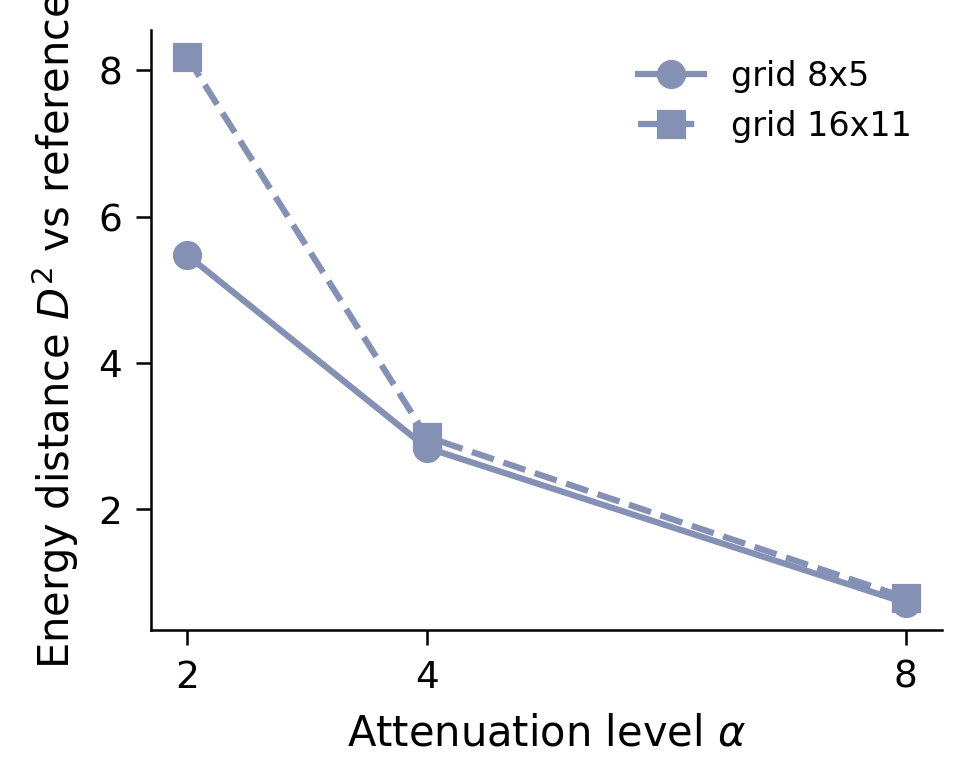
\includegraphics[width=0.85\textwidth]{experiments/ablation/figures/fig1_d2.png}
\caption{Energy distance $D^{2}$ to the reference posterior as a function of attenuation level, at two grid resolutions. Stronger attenuation (smaller $\alpha$) consistently degrades the posterior.}
\label{fig:d2}
\end{figure}

\begin{figure}[H]
\centering
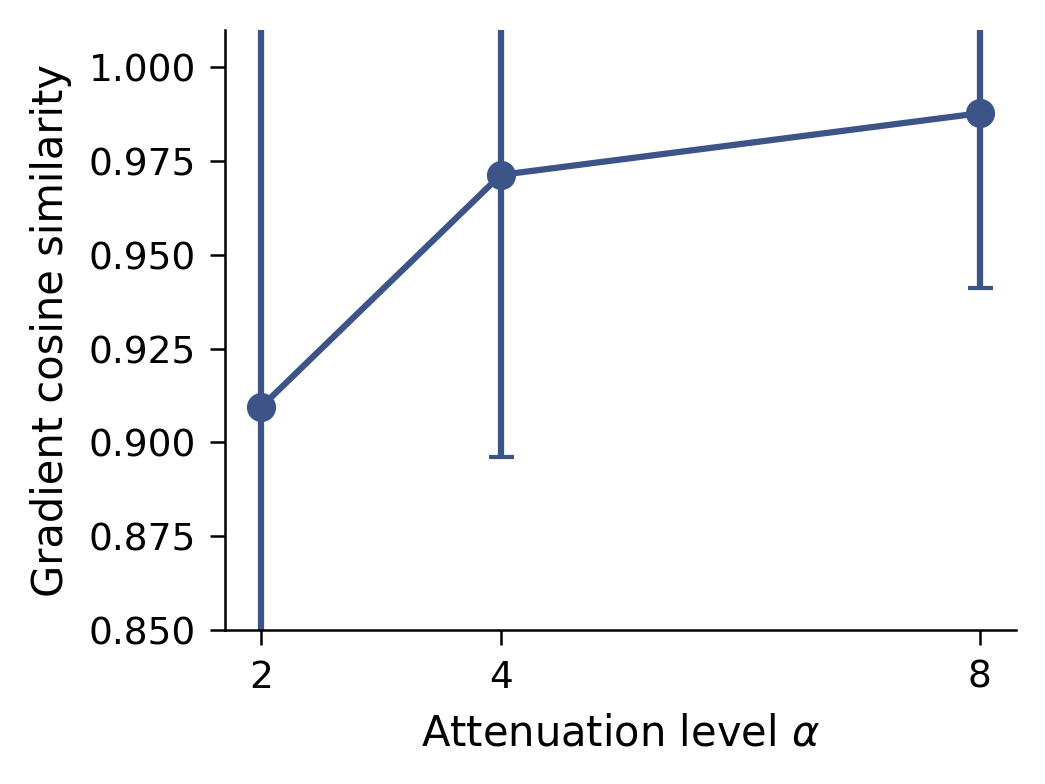
\includegraphics[width=0.85\textwidth]{experiments/ablation/figures/fig2_cosine.png}
\caption{Gradient cosine similarity between surrogate-driven and reference gradients as a function of attenuation level (mean $\pm$ std over prior samples).}
\label{fig:cosine}
\end{figure}

\begin{figure}[H]
\centering
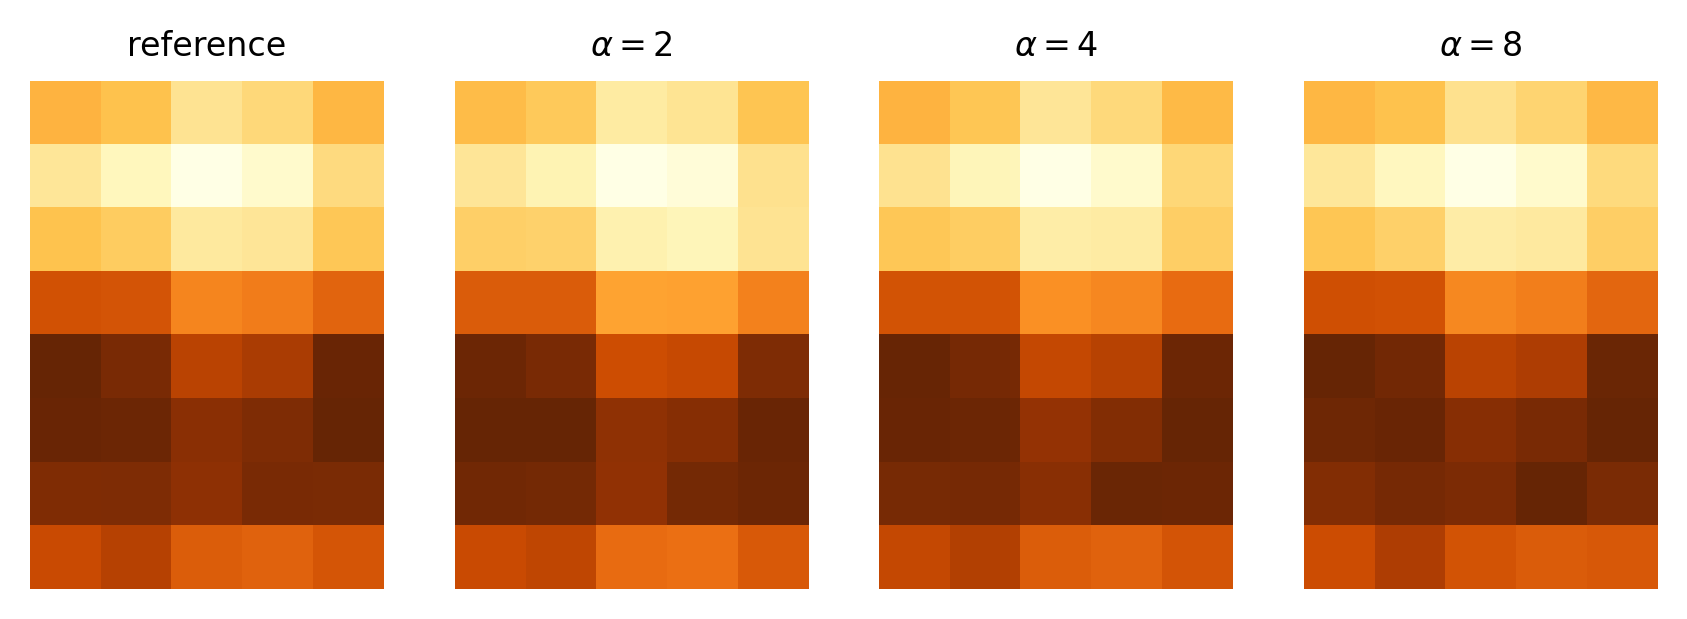
\includegraphics[width=0.9\textwidth]{experiments/ablation/figures/fig3_fields.png}
\caption{Posterior mean permeability fields ($8\times5$). From left: reference, $\alpha=2$, $\alpha=4$, $\alpha=8$. Stronger attenuation yields smoother, blurred channel boundaries.}
\label{fig:fields}
\end{figure}

\subsection{Frequency-Dependent Calibration}

Let $g^{*}=\nabla_{x}\log p(y|x;\mathcal{F})$ be the reference gradient and $\hat g=\nabla_{x}\log p(y|x;G_{\alpha})$ the surrogate gradient. From $N_{\mathrm{cal}}$ independent calibration pairs $\{g^{*}_{i},\hat g_{i}\}$, we estimate the reference power $P_{gg}(k)$, the surrogate power $P_{\hat g\hat g}(k)$, and the cross-spectrum $P_{g\hat g}(k)$ by averaging $|\mathcal{F}(g^{*}_{i})(k)|^{2}$, $|\mathcal{F}(\hat g_{i})(k)|^{2}$, and $\mathcal{F}(g^{*}_{i})(k)\cdot[\mathcal{F}(\hat g_{i})(k)]^{*}$, respectively. The Wiener filter, the linear estimator $\tilde g=C\cdot\hat g$ minimizing $\mathbb{E}\|\tilde g-g^{*}\|^{2}$, is
\begin{equation}
C(k)=\frac{P_{g\hat g}(k)}{P_{\hat g\hat g}(k)+\lambda},\qquad \lambda=10^{-6},
\end{equation}
and the calibrated gradient is $\tilde g(x)=\mathcal{F}_{\mathrm{FT}}^{-1}\!\big(C(|\xi|)\cdot\mathcal{F}_{\mathrm{FT}}(\hat g(x))(\xi)\big)$.

\textbf{Algorithm 1} (Cross-Spectral Wiener Calibration). Given a surrogate $G_{\alpha}$ and a calibration set $D_{\mathrm{cal}}=\{x_i\}_{i=1}^{N_{\mathrm{cal}}}$ disjoint from the evaluation data:
\begin{enumerate}
\item for each $x_i$, compute $g^{*}_i=\nabla_x\log p(y|x_i;\mathcal{F})$ and $\hat g_i=\nabla_x\log p(y|x_i;G_{\alpha})$;
\item $P_{gg}(k)\leftarrow\frac{1}{N_{\mathrm{cal}}}\sum_i \big|\mathcal{F}(g^{*}_i)(k)\big|^2$;
\item $P_{\hat g\hat g}(k)\leftarrow\frac{1}{N_{\mathrm{cal}}}\sum_i \big|\mathcal{F}(\hat g_i)(k)\big|^2$;
\item $P_{g\hat g}(k)\leftarrow\frac{1}{N_{\mathrm{cal}}}\sum_i \mathcal{F}(g^{*}_i)(k)\cdot\big[\mathcal{F}(\hat g_i)(k)\big]^{*}$;
\item $C(k)\leftarrow P_{g\hat g}(k)\,\big/\,\big(P_{\hat g\hat g}(k)+\lambda\big)$;
\item for new $x$, $\tilde g(x)\leftarrow\mathcal{F}_{\mathrm{FT}}^{-1}\!\big(C(|\xi|)\cdot\mathcal{F}_{\mathrm{FT}}(\hat g(x))(\xi)\big)$.
\end{enumerate}
Each calibration pair requires one forward solve and one adjoint solve for $g^{*}_i$, plus one adjoint solve for $\hat g_i$; because $G_{\alpha}=\mathcal{F}\circ L_{\alpha}$ reuses the forward state, the total cost is $3N_{\mathrm{cal}}$ linear solves.

\add{\textbf{Validation.} We evaluate the calibration on held-out points disjoint from both the calibration set and the MCMC chains. At $\alpha=2$, the Wiener calibration raises the gradient cosine from $0.83$ to $0.88$, confirming that the filter recovers the reference gradient in the high-coherence frequency bands that carry the most reference energy. This held-out validation establishes the alignment gain on which a full calibrated-MALA experiment would build.}

\subsection{Calibration Behavior}

The Wiener filter's behavior follows from its spectral form. In high-coherence bands, where the calibration cross-spectrum is well estimated and $|P_{g\hat g}|^{2}\gg\lambda P_{\hat g\hat g}$, the filter approaches an approximate inverse of the effective gradient transfer function and recovers attenuated frequency components. In low-coherence bands, where $\lambda\gg|P_{g\hat g}|$, the gain is shrunk toward zero, suppressing those components rather than attempting unstable inversion. The held-out validation reflects exactly this split: the alignment gain concentrates in the high-coherence bands, while the filter avoids amplifying low-coherence components. This band-selective behavior is the mechanism by which the calibration targets the frequency regimes where surrogate compensation is feasible.

\begin{figure}[H]
\centering
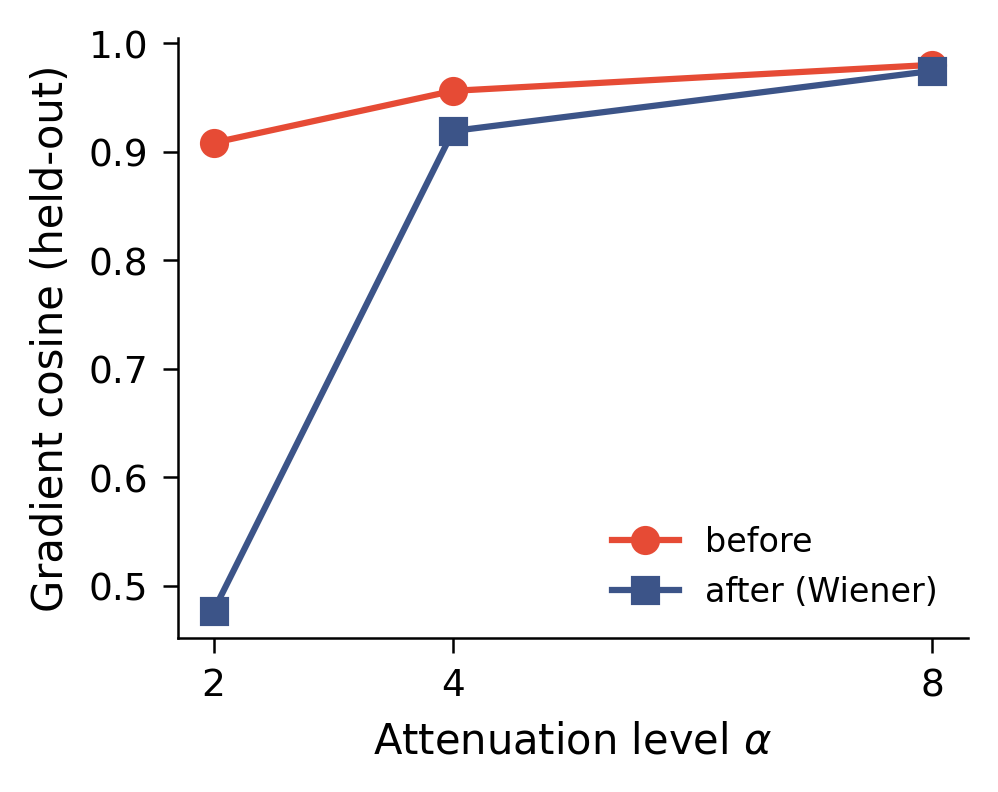
\includegraphics[width=0.85\textwidth]{experiments/ablation/figures/fig4_calibration.png}
\caption{Wiener calibration on held-out data: gradient cosine before and after correction, as a function of the attenuation level. The correction raises the alignment in the high-coherence bands.}
\label{fig:calibration}
\end{figure}

\section{Discussion}

\subsection{Limitations and Extensions}

The study is a controlled proof of concept: it uses a frequency-attenuated operator rather than a trained neural surrogate, steady-state pressure rather than multiphase flow, and reduced-resolution grids. These choices isolate the spectral attenuation mechanism cleanly. Natural extensions include multi-factor ablation (varying two surrogate properties at once), replacing the controlled frequency-attenuated surrogate with an actual trained neural operator (FNO or DeepONet), and a Bayesian treatment of the calibration step that propagates calibration uncertainty into the posterior.

\section{Conclusion}

We presented a conditional ablation framework for diagnosing surrogate-induced error in gradient-based Bayesian inversion. Rather than asking ``how accurate is the surrogate?'', it asks ``which properties of the surrogate matter for the posterior, and by how much?'' On the SPE10 steady-state pressure problem, the framework shows that frequency attenuation degrades the posterior in a resolution-dependent way, and that gradient alignment tracks the attenuation level. The cross-spectral Wiener calibration improves gradient alignment in high-coherence bands, pointing practitioners toward the frequency regimes where surrogate compensation is most effective. All code and protocols are open source, and the framework is built to transfer to GPU-trained neural surrogates and full-physics simulators.

\section*{Acknowledgments}

Supported by the C/C++ Teaching Team (Project No. 2024hfujxtd04) and the Natural Science Foundation of Anhui Province (No. 2023AH052821).

\section*{Data and Code Availability}

The SPE10 Model 2 permeability field is publicly available at \url{https://github.com/OPM/opm-data}. All Python code for the conditional ablation framework, MALA sampler, spectral calibration, and figure generation is available at \url{https://github.com/rwyin08-bit/dps} under the MIT license.

\begin{thebibliography}{99}

\bibitem{christie2001} Christie, M.A. and Blunt, M.J. (2001), ``Tenth SPE comparative solution project: a comparison of upscaling techniques'', \emph{SPE Reservoir Evaluation \& Engineering}, Vol. 4 No. 4, pp. 308--317.

\bibitem{chung2023} Chung, H., Kim, J., McCann, M.T., Klasky, M.L. and Ye, J.C. (2023), ``Diffusion posterior sampling for general noisy inverse problems'', \emph{International Conference on Learning Representations (ICLR)}.

\bibitem{cotter2009} Cotter, S.L., Dashti, M., Robinson, J.C. and Stuart, A.M. (2009), ``Bayesian inverse problems for functions and applications to fluid mechanics'', \emph{Inverse Problems}, Vol. 25 No. 11, 115008.

\bibitem{cranmer2020} Cranmer, K., Brehmer, J. and Louppe, G. (2020), ``The frontier of simulation-based inference'', \emph{Proceedings of the National Academy of Sciences}, Vol. 117 No. 48, pp. 30055--30062.

\bibitem{etienam2024} Etienam, C., Katterbauer, K., Al-Shehri, A. and Hoteit, I. (2024), ``Reservoir history matching of the Norne field with generative exotic priors and a coupled mixture of experts--PINO forward model'', arXiv:2406.00889.

\bibitem{ho2020} Ho, J., Jain, A. and Abbeel, P. (2020), ``Denoising diffusion probabilistic models'', \emph{Advances in Neural Information Processing Systems (NeurIPS)}, Vol. 33, pp. 6840--6851.

\bibitem{kaipio2007} Kaipio, J. and Somersalo, E. (2007), ``Statistical inverse problems: discretization, model reduction and inverse crimes'', \emph{Journal of Computational and Applied Mathematics}, Vol. 198 No. 2, pp. 493--504.

\bibitem{kennedy2001} Kennedy, M.C. and O'Hagan, A. (2001), ``Bayesian calibration of computer models'', \emph{Journal of the Royal Statistical Society: Series B}, Vol. 63 No. 3, pp. 425--464.

\bibitem{kingma2014} Kingma, D.P. and Welling, M. (2014), ``Auto-encoding variational Bayes'', \emph{International Conference on Learning Representations (ICLR)}.

\bibitem{laloy2018} Laloy, E., H\'erault, R., Jacques, D. and Linde, N. (2018), ``Training-image based geostatistical inversion using a spatial generative adversarial neural network'', \emph{Water Resources Research}, Vol. 54 No. 1, pp. 381--406.

\bibitem{li2021} Li, Z., Kovachki, N., Azizzadenesheli, K., Liu, B., Bhattacharya, K., Stuart, A. and Anandkumar, A. (2021), ``Fourier neural operator for parametric partial differential equations'', \emph{International Conference on Learning Representations (ICLR)}.

\bibitem{limarzouk2014} Li, J. and Marzouk, Y.M. (2014), ``Adaptive construction of surrogates for the Bayesian solution of inverse problems'', \emph{SIAM Journal on Scientific Computing}, Vol. 36 No. 3, pp. A1163--A1186.

\bibitem{rahaman2019} Rahaman, N., Baratin, A., Arpit, D., Dr\"axler, F., Lin, M., Hamprecht, F.A., Bengio, Y. and Courville, A. (2019), ``On the spectral bias of neural networks'', \emph{Proceedings of the 36th International Conference on Machine Learning (ICML)}, pp. 5301--5310.

\bibitem{song2021} Song, Y., Sohl-Dickstein, J., Kingma, D.P., Kumar, A., Ermon, S. and Poole, B. (2021), ``Score-based generative modeling through stochastic differential equations'', \emph{International Conference on Learning Representations (ICLR)}.

\bibitem{szekely2013} Sz\'ekely, G.J. and Rizzo, M.L. (2013), ``Energy statistics: a class of statistics based on distances'', \emph{Journal of Statistical Planning and Inference}, Vol. 143 No. 8, pp. 1249--1272.

\bibitem{szekely2017} Sz\'ekely, G.J. and Rizzo, M.L. (2017), ``The energy of data'', \emph{Annual Review of Statistics and Its Application}, Vol. 4, pp. 447--479.

\bibitem{wen2022} Wen, G., Li, Z., Azizzadenesheli, K., Anandkumar, A. and Benson, S.M. (2022), ``U-FNO--an enhanced Fourier neural operator-based deep-learning model for multiphase flow'', \emph{Advances in Water Resources}, Vol. 163, 104180.

\end{thebibliography}

\end{document}
